\documentclass[twoside]{book}

% Packages required by doxygen
\usepackage{fixltx2e}
\usepackage{calc}
\usepackage{doxygen}
\usepackage[export]{adjustbox} % also loads graphicx
\usepackage{graphicx}
\usepackage[utf8]{inputenc}
\usepackage{makeidx}
\usepackage{multicol}
\usepackage{multirow}
\PassOptionsToPackage{warn}{textcomp}
\usepackage{textcomp}
\usepackage[nointegrals]{wasysym}
\usepackage[table]{xcolor}

% Font selection
\usepackage[T1]{fontenc}
\usepackage[scaled=.90]{helvet}
\usepackage{courier}
\usepackage{amssymb}
\usepackage{sectsty}
\renewcommand{\familydefault}{\sfdefault}
\allsectionsfont{%
  \fontseries{bc}\selectfont%
  \color{darkgray}%
}
\renewcommand{\DoxyLabelFont}{%
  \fontseries{bc}\selectfont%
  \color{darkgray}%
}
\newcommand{\+}{\discretionary{\mbox{\scriptsize$\hookleftarrow$}}{}{}}

% Page & text layout
\usepackage{geometry}
\geometry{%
  a4paper,%
  top=2.5cm,%
  bottom=2.5cm,%
  left=2.5cm,%
  right=2.5cm%
}
\tolerance=750
\hfuzz=15pt
\hbadness=750
\setlength{\emergencystretch}{15pt}
\setlength{\parindent}{0cm}
\setlength{\parskip}{3ex plus 2ex minus 2ex}
\makeatletter
\renewcommand{\paragraph}{%
  \@startsection{paragraph}{4}{0ex}{-1.0ex}{1.0ex}{%
    \normalfont\normalsize\bfseries\SS@parafont%
  }%
}
\renewcommand{\subparagraph}{%
  \@startsection{subparagraph}{5}{0ex}{-1.0ex}{1.0ex}{%
    \normalfont\normalsize\bfseries\SS@subparafont%
  }%
}
\makeatother

% Headers & footers
\usepackage{fancyhdr}
\pagestyle{fancyplain}
\fancyhead[LE]{\fancyplain{}{\bfseries\thepage}}
\fancyhead[CE]{\fancyplain{}{}}
\fancyhead[RE]{\fancyplain{}{\bfseries\leftmark}}
\fancyhead[LO]{\fancyplain{}{\bfseries\rightmark}}
\fancyhead[CO]{\fancyplain{}{}}
\fancyhead[RO]{\fancyplain{}{\bfseries\thepage}}
\fancyfoot[LE]{\fancyplain{}{}}
\fancyfoot[CE]{\fancyplain{}{}}
\fancyfoot[RE]{\fancyplain{}{\bfseries\scriptsize Generated by Doxygen }}
\fancyfoot[LO]{\fancyplain{}{\bfseries\scriptsize Generated by Doxygen }}
\fancyfoot[CO]{\fancyplain{}{}}
\fancyfoot[RO]{\fancyplain{}{}}
\renewcommand{\footrulewidth}{0.4pt}
\renewcommand{\chaptermark}[1]{%
  \markboth{#1}{}%
}
\renewcommand{\sectionmark}[1]{%
  \markright{\thesection\ #1}%
}

% Indices & bibliography
\usepackage{natbib}
\usepackage[titles]{tocloft}
\setcounter{tocdepth}{3}
\setcounter{secnumdepth}{5}
\makeindex

% Hyperlinks (required, but should be loaded last)
\usepackage{ifpdf}
\ifpdf
  \usepackage[pdftex,pagebackref=true]{hyperref}
\else
  \usepackage[ps2pdf,pagebackref=true]{hyperref}
\fi
\hypersetup{%
  colorlinks=true,%
  linkcolor=blue,%
  citecolor=blue,%
  unicode%
}

% Custom commands
\newcommand{\clearemptydoublepage}{%
  \newpage{\pagestyle{empty}\cleardoublepage}%
}

\usepackage{caption}
\captionsetup{labelsep=space,justification=centering,font={bf},singlelinecheck=off,skip=4pt,position=top}

%===== C O N T E N T S =====

\begin{document}

% Titlepage & ToC
\hypersetup{pageanchor=false,
             bookmarksnumbered=true,
             pdfencoding=unicode
            }
\pagenumbering{alph}
\begin{titlepage}
\vspace*{7cm}
\begin{center}%
{\Large R\+T\+F\+EM }\\
\vspace*{1cm}
{\large Generated by Doxygen 1.8.14}\\
\end{center}
\end{titlepage}
\clearemptydoublepage
\pagenumbering{roman}
\tableofcontents
\clearemptydoublepage
\pagenumbering{arabic}
\hypersetup{pageanchor=true}

%--- Begin generated contents ---
\chapter{Hierarchical Index}
\section{Class Hierarchy}
This inheritance list is sorted roughly, but not completely, alphabetically\+:\begin{DoxyCompactList}
\item \contentsline{section}{rtfem\+:\+:F\+E\+M\+Assembler}{\pageref{classrtfem_1_1FEMAssembler}}{}
\item \contentsline{section}{rtfem\+:\+:F\+E\+M\+Model}{\pageref{classrtfem_1_1FEMModel}}{}
\item \contentsline{section}{rtfem\+:\+:F\+E\+M\+Solver}{\pageref{classrtfem_1_1FEMSolver}}{}
\item \contentsline{section}{rtfem\+:\+:Finite\+Element}{\pageref{classrtfem_1_1FiniteElement}}{}
\begin{DoxyCompactList}
\item \contentsline{section}{rtfem\+:\+:Tetrahedron\+Finite\+Element}{\pageref{classrtfem_1_1TetrahedronFiniteElement}}{}
\end{DoxyCompactList}
\item \contentsline{section}{rtfem\+:\+:Finite\+Element\+Solver}{\pageref{classrtfem_1_1FiniteElementSolver}}{}
\begin{DoxyCompactList}
\item \contentsline{section}{rtfem\+:\+:Tetrahedron\+Solver}{\pageref{classrtfem_1_1TetrahedronSolver}}{}
\end{DoxyCompactList}
\item \contentsline{section}{rtfem\+:\+:Finite\+Element\+Solver\+Data}{\pageref{structrtfem_1_1FiniteElementSolverData}}{}
\item \contentsline{section}{rtfem\+:\+:Global\+Stiffness\+Assembler}{\pageref{classrtfem_1_1GlobalStiffnessAssembler}}{}
\item \contentsline{section}{rtfem\+:\+:Material}{\pageref{structrtfem_1_1Material}}{}
\item \contentsline{section}{rtfem\+:\+:Matrix}{\pageref{classrtfem_1_1Matrix}}{}
\item \contentsline{section}{rtfem\+:\+:Matrix\+Dimension}{\pageref{structrtfem_1_1MatrixDimension}}{}
\item \contentsline{section}{rtfem\+:\+:Matrix\+Math}{\pageref{classrtfem_1_1MatrixMath}}{}
\item \contentsline{section}{rtfem\+:\+:Vector3}{\pageref{structrtfem_1_1Vector3}}{}
\item \contentsline{section}{rtfem\+:\+:Vertex}{\pageref{classrtfem_1_1Vertex}}{}
\end{DoxyCompactList}

\chapter{Class Index}
\section{Class List}
Here are the classes, structs, unions and interfaces with brief descriptions\+:\begin{DoxyCompactList}
\item\contentsline{section}{\hyperlink{classrtfem_1_1FEMAssembler}{rtfem\+::\+F\+E\+M\+Assembler} }{\pageref{classrtfem_1_1FEMAssembler}}{}
\item\contentsline{section}{\hyperlink{classrtfem_1_1FEMModel}{rtfem\+::\+F\+E\+M\+Model} }{\pageref{classrtfem_1_1FEMModel}}{}
\item\contentsline{section}{\hyperlink{classrtfem_1_1FEMSolver}{rtfem\+::\+F\+E\+M\+Solver} }{\pageref{classrtfem_1_1FEMSolver}}{}
\item\contentsline{section}{\hyperlink{classrtfem_1_1FiniteElement}{rtfem\+::\+Finite\+Element} }{\pageref{classrtfem_1_1FiniteElement}}{}
\item\contentsline{section}{\hyperlink{classrtfem_1_1FiniteElementSolver}{rtfem\+::\+Finite\+Element\+Solver} }{\pageref{classrtfem_1_1FiniteElementSolver}}{}
\item\contentsline{section}{\hyperlink{structrtfem_1_1FiniteElementSolverData}{rtfem\+::\+Finite\+Element\+Solver\+Data} }{\pageref{structrtfem_1_1FiniteElementSolverData}}{}
\item\contentsline{section}{\hyperlink{classrtfem_1_1GlobalStiffnessAssembler}{rtfem\+::\+Global\+Stiffness\+Assembler} }{\pageref{classrtfem_1_1GlobalStiffnessAssembler}}{}
\item\contentsline{section}{\hyperlink{structrtfem_1_1Material}{rtfem\+::\+Material} }{\pageref{structrtfem_1_1Material}}{}
\item\contentsline{section}{\hyperlink{classrtfem_1_1Matrix}{rtfem\+::\+Matrix} }{\pageref{classrtfem_1_1Matrix}}{}
\item\contentsline{section}{\hyperlink{structrtfem_1_1MatrixDimension}{rtfem\+::\+Matrix\+Dimension} }{\pageref{structrtfem_1_1MatrixDimension}}{}
\item\contentsline{section}{\hyperlink{classrtfem_1_1MatrixMath}{rtfem\+::\+Matrix\+Math} }{\pageref{classrtfem_1_1MatrixMath}}{}
\item\contentsline{section}{\hyperlink{classrtfem_1_1TetrahedronFiniteElement}{rtfem\+::\+Tetrahedron\+Finite\+Element} }{\pageref{classrtfem_1_1TetrahedronFiniteElement}}{}
\item\contentsline{section}{\hyperlink{classrtfem_1_1TetrahedronSolver}{rtfem\+::\+Tetrahedron\+Solver} }{\pageref{classrtfem_1_1TetrahedronSolver}}{}
\item\contentsline{section}{\hyperlink{structrtfem_1_1Vector3}{rtfem\+::\+Vector3} }{\pageref{structrtfem_1_1Vector3}}{}
\item\contentsline{section}{\hyperlink{classrtfem_1_1Vertex}{rtfem\+::\+Vertex} }{\pageref{classrtfem_1_1Vertex}}{}
\end{DoxyCompactList}

\chapter{Class Documentation}
\hypertarget{classrtfem_1_1FEMAssembler}{}\section{rtfem\+:\+:F\+E\+M\+Assembler Class Reference}
\label{classrtfem_1_1FEMAssembler}\index{rtfem\+::\+F\+E\+M\+Assembler@{rtfem\+::\+F\+E\+M\+Assembler}}
\subsection*{Public Member Functions}
\begin{DoxyCompactItemize}
\item 
\mbox{\Hypertarget{classrtfem_1_1FEMAssembler_acfa55c7a2eb8a1c7b1e3b5ffc810c3b0}\label{classrtfem_1_1FEMAssembler_acfa55c7a2eb8a1c7b1e3b5ffc810c3b0}} 
\hyperlink{classrtfem_1_1Matrix}{Matrix} {\bfseries Compute\+Global\+Stiffness} (const std\+::shared\+\_\+ptr$<$ \hyperlink{classrtfem_1_1FEMModel}{F\+E\+M\+Model} $>$ fem\+\_\+model)
\end{DoxyCompactItemize}


The documentation for this class was generated from the following files\+:\begin{DoxyCompactItemize}
\item 
/home/samba/ciecierskij/programming/rt\+\_\+fem/sources/include/\+R\+T\+F\+E\+M/\+F\+E\+M/\+Solver/F\+E\+M\+Assembler.\+h\item 
/home/samba/ciecierskij/programming/rt\+\_\+fem/sources/src/\+R\+T\+F\+E\+M/\+F\+E\+M/\+Solver/F\+E\+M\+Assembler.\+cpp\end{DoxyCompactItemize}

\hypertarget{classrtfem_1_1FEMModel}{}\section{rtfem\+:\+:F\+E\+M\+Model Class Reference}
\label{classrtfem_1_1FEMModel}\index{rtfem\+::\+F\+E\+M\+Model@{rtfem\+::\+F\+E\+M\+Model}}


{\ttfamily \#include $<$F\+E\+M\+Model.\+h$>$}

\subsection*{Public Member Functions}
\begin{DoxyCompactItemize}
\item 
\mbox{\Hypertarget{classrtfem_1_1FEMModel_ad42ae0bcf7a820c8c0a0bba6ebe56d12}\label{classrtfem_1_1FEMModel_ad42ae0bcf7a820c8c0a0bba6ebe56d12}} 
{\bfseries F\+E\+M\+Model} (std\+::vector$<$ std\+::shared\+\_\+ptr$<$ \hyperlink{classrtfem_1_1FiniteElement}{Finite\+Element} $>$$>$ \&finite\+\_\+elements\+\_\+, std\+::vector$<$ std\+::shared\+\_\+ptr$<$ \hyperlink{classrtfem_1_1Vertex}{Vertex} $>$$>$ \&vertices\+\_\+, const \hyperlink{structrtfem_1_1Material}{Material} \&\&material)
\item 
\mbox{\Hypertarget{classrtfem_1_1FEMModel_aef907014b922f5815df70d620761bb1c}\label{classrtfem_1_1FEMModel_aef907014b922f5815df70d620761bb1c}} 
const std\+::vector$<$ std\+::shared\+\_\+ptr$<$ \hyperlink{classrtfem_1_1FiniteElement}{Finite\+Element} $>$ $>$ \& {\bfseries finite\+\_\+elements} () const
\item 
\mbox{\Hypertarget{classrtfem_1_1FEMModel_a97bfc0a7d29557bebe4014ceb2f74b13}\label{classrtfem_1_1FEMModel_a97bfc0a7d29557bebe4014ceb2f74b13}} 
const std\+::vector$<$ std\+::shared\+\_\+ptr$<$ \hyperlink{classrtfem_1_1Vertex}{Vertex} $>$ $>$ \& {\bfseries vertices} () const
\item 
\mbox{\Hypertarget{classrtfem_1_1FEMModel_ae5582a990cf4d4c8cda4f7cc44e947ba}\label{classrtfem_1_1FEMModel_ae5582a990cf4d4c8cda4f7cc44e947ba}} 
\hyperlink{structrtfem_1_1Material}{Material} \& {\bfseries material} ()
\item 
\mbox{\Hypertarget{classrtfem_1_1FEMModel_a20227bb6ddae580e8f4251b4b0c31edc}\label{classrtfem_1_1FEMModel_a20227bb6ddae580e8f4251b4b0c31edc}} 
U\+Int {\bfseries Vertex\+Count} ()
\item 
\mbox{\Hypertarget{classrtfem_1_1FEMModel_a9eeb90bb47a133bba20c39d95c073fbc}\label{classrtfem_1_1FEMModel_a9eeb90bb47a133bba20c39d95c073fbc}} 
U\+Int {\bfseries Finite\+Element\+Count} ()
\end{DoxyCompactItemize}


\subsection{Detailed Description}
\hyperlink{classrtfem_1_1FEMModel}{F\+E\+M\+Model} contains model of a single connected object. T\+O\+DO\+: What does it mean $^\wedge$ ? 

The documentation for this class was generated from the following files\+:\begin{DoxyCompactItemize}
\item 
/home/samba/ciecierskij/programming/rt\+\_\+fem/sources/include/\+R\+T\+F\+E\+M/\+F\+E\+M/F\+E\+M\+Model.\+h\item 
/home/samba/ciecierskij/programming/rt\+\_\+fem/sources/src/\+R\+T\+F\+E\+M/\+F\+E\+M/F\+E\+M\+Model.\+cpp\end{DoxyCompactItemize}

\hypertarget{classrtfem_1_1FEMSolver}{}\section{rtfem\+:\+:F\+E\+M\+Solver Class Reference}
\label{classrtfem_1_1FEMSolver}\index{rtfem\+::\+F\+E\+M\+Solver@{rtfem\+::\+F\+E\+M\+Solver}}
\subsection*{Public Member Functions}
\begin{DoxyCompactItemize}
\item 
\mbox{\Hypertarget{classrtfem_1_1FEMSolver_ad1d4aa21a4a8e86b5e0dbc8f9f76b583}\label{classrtfem_1_1FEMSolver_ad1d4aa21a4a8e86b5e0dbc8f9f76b583}} 
{\bfseries F\+E\+M\+Solver} (const Constitutive\+Solver\+Type \&\&constitutive\+\_\+solver\+\_\+type, const Geometry\+Solver\+Type \&\&geometry\+\_\+solver\+\_\+type, const Analysis\+Solver\+Type \&\&analysis\+\_\+solver\+\_\+type)
\item 
\mbox{\Hypertarget{classrtfem_1_1FEMSolver_afa39adf6bf64fba7cff1d0ccac754ed3}\label{classrtfem_1_1FEMSolver_afa39adf6bf64fba7cff1d0ccac754ed3}} 
const Constitutive\+Solver\+Type \& {\bfseries constitutive\+\_\+solver\+\_\+type} ()
\item 
\mbox{\Hypertarget{classrtfem_1_1FEMSolver_a52048bd67869bb0e65d378f4b88cd226}\label{classrtfem_1_1FEMSolver_a52048bd67869bb0e65d378f4b88cd226}} 
const Geometry\+Solver\+Type \& {\bfseries geometry\+\_\+solver\+\_\+type} ()
\item 
\mbox{\Hypertarget{classrtfem_1_1FEMSolver_a15ddb99888344eab615524eb55ec88a6}\label{classrtfem_1_1FEMSolver_a15ddb99888344eab615524eb55ec88a6}} 
const Analysis\+Solver\+Type \& {\bfseries analysis\+\_\+solver\+\_\+type} ()
\item 
\mbox{\Hypertarget{classrtfem_1_1FEMSolver_a02fc9d1a5925b971aac2e24935800c64}\label{classrtfem_1_1FEMSolver_a02fc9d1a5925b971aac2e24935800c64}} 
void {\bfseries Solve} (const std\+::shared\+\_\+ptr$<$ \hyperlink{classrtfem_1_1FEMModel}{F\+E\+M\+Model} $>$ fem\+\_\+model)
\end{DoxyCompactItemize}


The documentation for this class was generated from the following files\+:\begin{DoxyCompactItemize}
\item 
/home/samba/ciecierskij/programming/rt\+\_\+fem/sources/include/\+R\+T\+F\+E\+M/\+F\+E\+M/\+Solver/F\+E\+M\+Solver.\+h\item 
/home/samba/ciecierskij/programming/rt\+\_\+fem/sources/src/\+R\+T\+F\+E\+M/\+F\+E\+M/\+Solver/F\+E\+M\+Solver.\+cpp\end{DoxyCompactItemize}

\hypertarget{classrtfem_1_1FiniteElement}{}\section{rtfem\+:\+:Finite\+Element Class Reference}
\label{classrtfem_1_1FiniteElement}\index{rtfem\+::\+Finite\+Element@{rtfem\+::\+Finite\+Element}}


{\ttfamily \#include $<$Finite\+Element.\+h$>$}

Inheritance diagram for rtfem\+:\+:Finite\+Element\+:\begin{figure}[H]
\begin{center}
\leavevmode
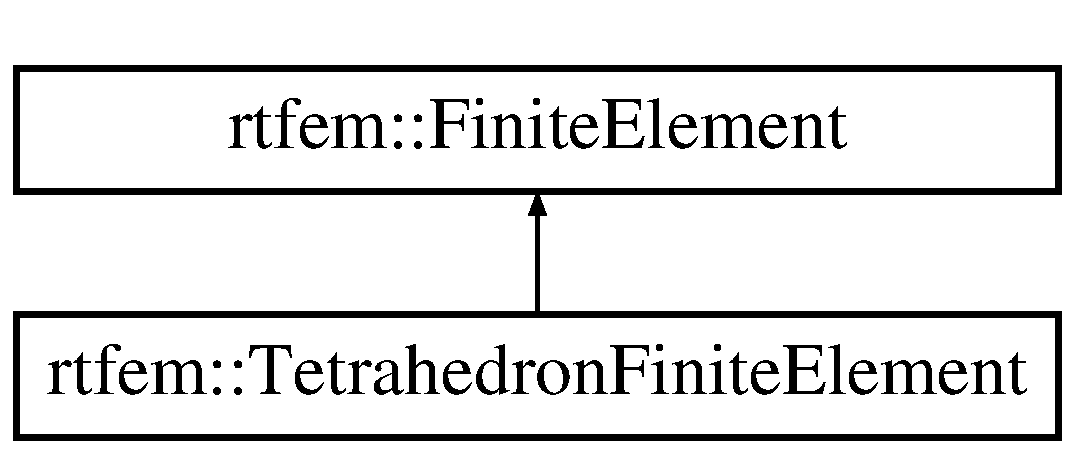
\includegraphics[height=2.000000cm]{classrtfem_1_1FiniteElement}
\end{center}
\end{figure}
\subsection*{Public Member Functions}
\begin{DoxyCompactItemize}
\item 
\mbox{\Hypertarget{classrtfem_1_1FiniteElement_ad1fd028110f56384d5e7d3660699bdd2}\label{classrtfem_1_1FiniteElement_ad1fd028110f56384d5e7d3660699bdd2}} 
{\bfseries Finite\+Element} (const Finite\+Element\+Type \&\&type)
\item 
\mbox{\Hypertarget{classrtfem_1_1FiniteElement_a5564187e7bd5d933517601ae2a67a7fd}\label{classrtfem_1_1FiniteElement_a5564187e7bd5d933517601ae2a67a7fd}} 
const Finite\+Element\+Type \& {\bfseries type} () const
\item 
\mbox{\Hypertarget{classrtfem_1_1FiniteElement_a2b330c717adf34307bca11ccb6fc1876}\label{classrtfem_1_1FiniteElement_a2b330c717adf34307bca11ccb6fc1876}} 
const std\+::vector$<$ std\+::shared\+\_\+ptr$<$ \hyperlink{classrtfem_1_1Vertex}{Vertex} $>$ $>$ \& {\bfseries vertices} ()
\item 
\mbox{\Hypertarget{classrtfem_1_1FiniteElement_a87155114b3992082f3c719ec5e2ec322}\label{classrtfem_1_1FiniteElement_a87155114b3992082f3c719ec5e2ec322}} 
virtual U\+Int {\bfseries Get\+Vertex\+Count} () const =0
\end{DoxyCompactItemize}
\subsection*{Protected Attributes}
\begin{DoxyCompactItemize}
\item 
\mbox{\Hypertarget{classrtfem_1_1FiniteElement_aa86ce90533ec663952e6d08890eae589}\label{classrtfem_1_1FiniteElement_aa86ce90533ec663952e6d08890eae589}} 
std\+::vector$<$ std\+::shared\+\_\+ptr$<$ \hyperlink{classrtfem_1_1Vertex}{Vertex} $>$ $>$ {\bfseries vertices\+\_\+}
\end{DoxyCompactItemize}


\subsection{Detailed Description}
Abstract class for Finite Element. 

The documentation for this class was generated from the following files\+:\begin{DoxyCompactItemize}
\item 
/home/samba/ciecierskij/programming/rt\+\_\+fem/sources/include/\+R\+T\+F\+E\+M/\+F\+E\+M/Finite\+Element.\+h\item 
/home/samba/ciecierskij/programming/rt\+\_\+fem/sources/src/\+R\+T\+F\+E\+M/\+F\+E\+M/Finite\+Element.\+cpp\end{DoxyCompactItemize}

\hypertarget{classrtfem_1_1FiniteElementSolver}{}\section{rtfem\+:\+:Finite\+Element\+Solver Class Reference}
\label{classrtfem_1_1FiniteElementSolver}\index{rtfem\+::\+Finite\+Element\+Solver@{rtfem\+::\+Finite\+Element\+Solver}}


{\ttfamily \#include $<$Finite\+Element\+Solver.\+h$>$}

Inheritance diagram for rtfem\+:\+:Finite\+Element\+Solver\+:\begin{figure}[H]
\begin{center}
\leavevmode
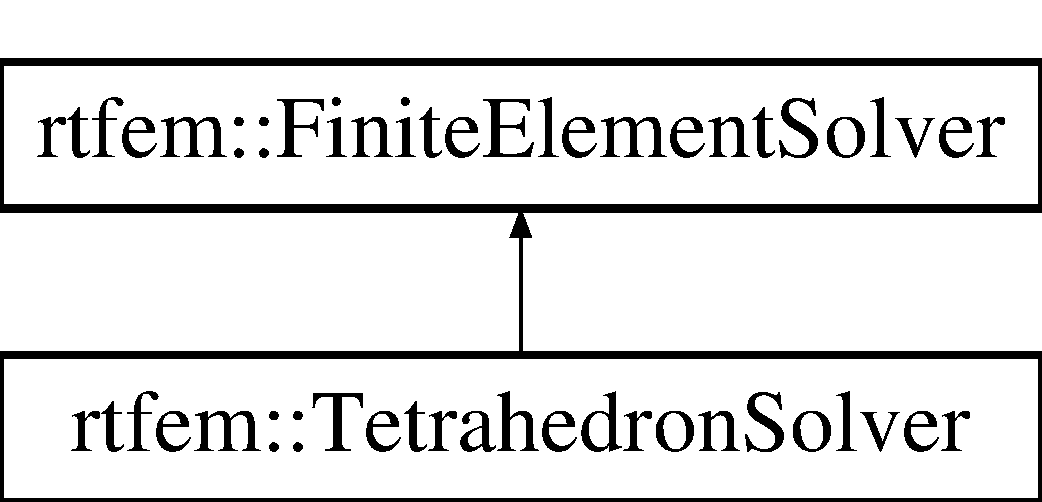
\includegraphics[height=2.000000cm]{classrtfem_1_1FiniteElementSolver}
\end{center}
\end{figure}
\subsection*{Public Member Functions}
\begin{DoxyCompactItemize}
\item 
\mbox{\Hypertarget{classrtfem_1_1FiniteElementSolver_a4aff399cbe0b356b0187e4c082e17b2c}\label{classrtfem_1_1FiniteElementSolver_a4aff399cbe0b356b0187e4c082e17b2c}} 
virtual \hyperlink{structrtfem_1_1FiniteElementSolverData}{Finite\+Element\+Solver\+Data} {\bfseries Solve} (std\+::shared\+\_\+ptr$<$ \hyperlink{classrtfem_1_1FiniteElement}{Finite\+Element} $>$ finite\+\_\+element)=0
\end{DoxyCompactItemize}


\subsection{Detailed Description}
Computes \hyperlink{structrtfem_1_1FiniteElementSolverData}{Finite\+Element\+Solver\+Data} for a given \hyperlink{classrtfem_1_1FiniteElement}{Finite\+Element}. 

The documentation for this class was generated from the following files\+:\begin{DoxyCompactItemize}
\item 
/home/samba/ciecierskij/programming/rt\+\_\+fem/sources/include/\+R\+T\+F\+E\+M/\+F\+E\+M/\+Solver/Finite\+Element\+Solver.\+h\item 
/home/samba/ciecierskij/programming/rt\+\_\+fem/sources/src/\+R\+T\+F\+E\+M/\+F\+E\+M/\+Solver/Finite\+Element\+Solver.\+cpp\end{DoxyCompactItemize}

\hypertarget{structrtfem_1_1FiniteElementSolverData}{}\section{rtfem\+:\+:Finite\+Element\+Solver\+Data Struct Reference}
\label{structrtfem_1_1FiniteElementSolverData}\index{rtfem\+::\+Finite\+Element\+Solver\+Data@{rtfem\+::\+Finite\+Element\+Solver\+Data}}


{\ttfamily \#include $<$Finite\+Element\+Solver.\+h$>$}

\subsection*{Public Attributes}
\begin{DoxyCompactItemize}
\item 
\mbox{\Hypertarget{structrtfem_1_1FiniteElementSolverData_a4e89fa242b0bcf6709f9ee69856133ff}\label{structrtfem_1_1FiniteElementSolverData_a4e89fa242b0bcf6709f9ee69856133ff}} 
Float {\bfseries volume}
\item 
\mbox{\Hypertarget{structrtfem_1_1FiniteElementSolverData_a128d2d84f8115132b9cf28e5543777a4}\label{structrtfem_1_1FiniteElementSolverData_a128d2d84f8115132b9cf28e5543777a4}} 
\hyperlink{classrtfem_1_1Matrix}{Matrix} {\bfseries shape\+\_\+matrix}
\item 
\mbox{\Hypertarget{structrtfem_1_1FiniteElementSolverData_a0f97fcf6d2d8d61f53c5a73c935e586d}\label{structrtfem_1_1FiniteElementSolverData_a0f97fcf6d2d8d61f53c5a73c935e586d}} 
\hyperlink{classrtfem_1_1Matrix}{Matrix} {\bfseries geometry\+\_\+matrix}
\end{DoxyCompactItemize}


\subsection{Detailed Description}
Contains\+: Volume. Shape \hyperlink{classrtfem_1_1Matrix}{Matrix} Geometry \hyperlink{classrtfem_1_1Matrix}{Matrix}

Coordinates\+: x2 is assumed to point \textquotesingle{}up\textquotesingle{} 

The documentation for this struct was generated from the following file\+:\begin{DoxyCompactItemize}
\item 
/home/samba/ciecierskij/programming/rt\+\_\+fem/sources/include/\+R\+T\+F\+E\+M/\+F\+E\+M/\+Solver/Finite\+Element\+Solver.\+h\end{DoxyCompactItemize}

\hypertarget{classrtfem_1_1GlobalStiffnessAssembler}{}\section{rtfem\+:\+:Global\+Stiffness\+Assembler Class Reference}
\label{classrtfem_1_1GlobalStiffnessAssembler}\index{rtfem\+::\+Global\+Stiffness\+Assembler@{rtfem\+::\+Global\+Stiffness\+Assembler}}


{\ttfamily \#include $<$Global\+Stiffness\+Assembler.\+h$>$}

\subsection*{Public Member Functions}
\begin{DoxyCompactItemize}
\item 
\hyperlink{classrtfem_1_1Matrix}{Matrix} \hyperlink{classrtfem_1_1GlobalStiffnessAssembler_a1da0902be1ae9e0fe7a5f7d2645597e3}{Compute} (const std\+::shared\+\_\+ptr$<$ \hyperlink{classrtfem_1_1FEMModel}{F\+E\+M\+Model} $>$ fem\+\_\+model)
\end{DoxyCompactItemize}


\subsection{Detailed Description}
Local Stiffness \hyperlink{classrtfem_1_1Matrix}{Matrix} (k) is the stiffness of each element \mbox{[}3\+Ne x 3\+Ne\mbox{]} e.\+g. for Tetrahedron (Ne = 3) thus\+: (dim = \mbox{[}12 x 12\mbox{]})

Global Stiffness \hyperlink{classrtfem_1_1Matrix}{Matrix} (K) is the stiffness of entire F\+EM Model \mbox{[}3N x 3N\mbox{]} e.\+g. For 9 vertices (dim = \mbox{[}27 x 27\mbox{]})

Partial Global Stiffness \hyperlink{classrtfem_1_1Matrix}{Matrix} (Ke) is the matrix of dimension equal to Global Stiffness but filled with only Local Stiffness data. 

\subsection{Member Function Documentation}
\mbox{\Hypertarget{classrtfem_1_1GlobalStiffnessAssembler_a1da0902be1ae9e0fe7a5f7d2645597e3}\label{classrtfem_1_1GlobalStiffnessAssembler_a1da0902be1ae9e0fe7a5f7d2645597e3}} 
\index{rtfem\+::\+Global\+Stiffness\+Assembler@{rtfem\+::\+Global\+Stiffness\+Assembler}!Compute@{Compute}}
\index{Compute@{Compute}!rtfem\+::\+Global\+Stiffness\+Assembler@{rtfem\+::\+Global\+Stiffness\+Assembler}}
\subsubsection{\texorpdfstring{Compute()}{Compute()}}
{\footnotesize\ttfamily \hyperlink{classrtfem_1_1Matrix}{Matrix} rtfem\+::\+Global\+Stiffness\+Assembler\+::\+Compute (\begin{DoxyParamCaption}\item[{const std\+::shared\+\_\+ptr$<$ \hyperlink{classrtfem_1_1FEMModel}{F\+E\+M\+Model} $>$}]{fem\+\_\+model }\end{DoxyParamCaption})}

Computes Global Stiffness \hyperlink{classrtfem_1_1Matrix}{Matrix} (K). \begin{DoxyVerb} 1) Computes Constitutive Matrix (C)
 2) Computes Geometry Matrix (B) for each Finite Element
 3) Computes Local Stiffness (k) for each Finite Element
     - Using Constitutive Matrix and Geometry Matrix.
 4) Assembles all Local Stiffness matrices into Global Stiffness Matrix (K)
\end{DoxyVerb}



\begin{DoxyParams}{Parameters}
{\em fem\+\_\+model} & \\
\hline
\end{DoxyParams}
\begin{DoxyReturn}{Returns}

\end{DoxyReturn}


The documentation for this class was generated from the following files\+:\begin{DoxyCompactItemize}
\item 
/home/samba/ciecierskij/programming/rt\+\_\+fem/sources/include/\+R\+T\+F\+E\+M/\+F\+E\+M/\+Solver/Global\+Stiffness\+Assembler.\+h\item 
/home/samba/ciecierskij/programming/rt\+\_\+fem/sources/src/\+R\+T\+F\+E\+M/\+F\+E\+M/\+Solver/Global\+Stiffness\+Assembler.\+cpp\end{DoxyCompactItemize}

\hypertarget{structrtfem_1_1Material}{}\section{rtfem\+:\+:Material Struct Reference}
\label{structrtfem_1_1Material}\index{rtfem\+::\+Material@{rtfem\+::\+Material}}


{\ttfamily \#include $<$Material.\+h$>$}

\subsection*{Public Attributes}
\begin{DoxyCompactItemize}
\item 
\mbox{\Hypertarget{structrtfem_1_1Material_a5743ec415411f1d7861938245e33ba7f}\label{structrtfem_1_1Material_a5743ec415411f1d7861938245e33ba7f}} 
Float {\bfseries young\+\_\+modulus}
\item 
\mbox{\Hypertarget{structrtfem_1_1Material_a6e6d121609178a7ed876fc8be303bad9}\label{structrtfem_1_1Material_a6e6d121609178a7ed876fc8be303bad9}} 
Float {\bfseries poisson\+\_\+coefficient}
\end{DoxyCompactItemize}


\subsection{Detailed Description}
One \hyperlink{structrtfem_1_1Material}{Material} per \hyperlink{classrtfem_1_1FEMModel}{F\+E\+M\+Model}

T\+O\+DO\+: Bounds of material properties (e.\+g. poisson \mbox{[}0, 0.\+5\mbox{]}

T\+O\+DO\+: \hyperlink{structrtfem_1_1Material}{Material} could be bound to each \hyperlink{classrtfem_1_1FiniteElement}{Finite\+Element} seperatly, allowing for \textquotesingle{}illusion\textquotesingle{} of composite materials. That would require computing Constitutive \hyperlink{classrtfem_1_1Matrix}{Matrix} for each \hyperlink{classrtfem_1_1FiniteElement}{Finite\+Element}. 

The documentation for this struct was generated from the following file\+:\begin{DoxyCompactItemize}
\item 
/home/samba/ciecierskij/programming/rt\+\_\+fem/sources/include/\+R\+T\+F\+E\+M/\+F\+E\+M/Material.\+h\end{DoxyCompactItemize}

\hypertarget{classrtfem_1_1Matrix}{}\section{rtfem\+:\+:Matrix Class Reference}
\label{classrtfem_1_1Matrix}\index{rtfem\+::\+Matrix@{rtfem\+::\+Matrix}}
\subsection*{Public Member Functions}
\begin{DoxyCompactItemize}
\item 
\hyperlink{classrtfem_1_1Matrix_af6122e873f49182e48f95a2d3a91f5ba}{Matrix} (U\+Int row\+\_\+count, U\+Int column\+\_\+count)
\item 
\mbox{\Hypertarget{classrtfem_1_1Matrix_a71423cbb4c6cbe0c46bb4a8cc4e87063}\label{classrtfem_1_1Matrix_a71423cbb4c6cbe0c46bb4a8cc4e87063}} 
{\bfseries Matrix} (const \hyperlink{structrtfem_1_1MatrixDimension}{Matrix\+Dimension} \&\&matrix\+\_\+dimension)
\item 
\mbox{\Hypertarget{classrtfem_1_1Matrix_a931e8b928bb80eeab0b3f32ab8cf7634}\label{classrtfem_1_1Matrix_a931e8b928bb80eeab0b3f32ab8cf7634}} 
const \hyperlink{structrtfem_1_1MatrixDimension}{Matrix\+Dimension} \& {\bfseries dimensions} () const
\item 
std\+::vector$<$ Float $>$ \& \hyperlink{classrtfem_1_1Matrix_afc502c2c20deb2a11562f6d55217093b}{operator\mbox{[}$\,$\mbox{]}} (U\+Int i)
\item 
\mbox{\Hypertarget{classrtfem_1_1Matrix_a799f80a8ff3f0794814e848fb90d2a1e}\label{classrtfem_1_1Matrix_a799f80a8ff3f0794814e848fb90d2a1e}} 
const std\+::vector$<$ Float $>$ \& {\bfseries operator\mbox{[}$\,$\mbox{]}} (U\+Int i) const
\item 
std\+::vector$<$ Float $>$ \& \hyperlink{classrtfem_1_1Matrix_acbb68e60ae9007c824c058b1e10825a5}{Get\+Row} (U\+Int i)
\item 
\mbox{\Hypertarget{classrtfem_1_1Matrix_a892b9524461866bd8cdb291ff608aa00}\label{classrtfem_1_1Matrix_a892b9524461866bd8cdb291ff608aa00}} 
const std\+::vector$<$ Float $>$ \& {\bfseries Get\+Row} (U\+Int i) const
\end{DoxyCompactItemize}


\subsection{Constructor \& Destructor Documentation}
\mbox{\Hypertarget{classrtfem_1_1Matrix_af6122e873f49182e48f95a2d3a91f5ba}\label{classrtfem_1_1Matrix_af6122e873f49182e48f95a2d3a91f5ba}} 
\index{rtfem\+::\+Matrix@{rtfem\+::\+Matrix}!Matrix@{Matrix}}
\index{Matrix@{Matrix}!rtfem\+::\+Matrix@{rtfem\+::\+Matrix}}
\subsubsection{\texorpdfstring{Matrix()}{Matrix()}}
{\footnotesize\ttfamily rtfem\+::\+Matrix\+::\+Matrix (\begin{DoxyParamCaption}\item[{U\+Int}]{row\+\_\+count,  }\item[{U\+Int}]{column\+\_\+count }\end{DoxyParamCaption})}

Creates \hyperlink{classrtfem_1_1Matrix}{Matrix} with row\+\_\+count rows and column\+\_\+count columns 
\begin{DoxyParams}{Parameters}
{\em row\+\_\+count} & \\
\hline
{\em column\+\_\+count} & \\
\hline
\end{DoxyParams}


\subsection{Member Function Documentation}
\mbox{\Hypertarget{classrtfem_1_1Matrix_acbb68e60ae9007c824c058b1e10825a5}\label{classrtfem_1_1Matrix_acbb68e60ae9007c824c058b1e10825a5}} 
\index{rtfem\+::\+Matrix@{rtfem\+::\+Matrix}!Get\+Row@{Get\+Row}}
\index{Get\+Row@{Get\+Row}!rtfem\+::\+Matrix@{rtfem\+::\+Matrix}}
\subsubsection{\texorpdfstring{Get\+Row()}{GetRow()}}
{\footnotesize\ttfamily std\+::vector$<$ Float $>$ \& rtfem\+::\+Matrix\+::\+Get\+Row (\begin{DoxyParamCaption}\item[{U\+Int}]{i }\end{DoxyParamCaption})}

Returns i-\/th row. 
\begin{DoxyParams}{Parameters}
{\em i} & \\
\hline
\end{DoxyParams}
\begin{DoxyReturn}{Returns}

\end{DoxyReturn}
\mbox{\Hypertarget{classrtfem_1_1Matrix_afc502c2c20deb2a11562f6d55217093b}\label{classrtfem_1_1Matrix_afc502c2c20deb2a11562f6d55217093b}} 
\index{rtfem\+::\+Matrix@{rtfem\+::\+Matrix}!operator\mbox{[}\mbox{]}@{operator[]}}
\index{operator\mbox{[}\mbox{]}@{operator[]}!rtfem\+::\+Matrix@{rtfem\+::\+Matrix}}
\subsubsection{\texorpdfstring{operator[]()}{operator[]()}}
{\footnotesize\ttfamily std\+::vector$<$ Float $>$ \& rtfem\+::\+Matrix\+::operator\mbox{[}$\,$\mbox{]} (\begin{DoxyParamCaption}\item[{U\+Int}]{i }\end{DoxyParamCaption})}

Returns i-\/th row. 
\begin{DoxyParams}{Parameters}
{\em i} & \\
\hline
\end{DoxyParams}
\begin{DoxyReturn}{Returns}

\end{DoxyReturn}


The documentation for this class was generated from the following files\+:\begin{DoxyCompactItemize}
\item 
/home/samba/ciecierskij/programming/rt\+\_\+fem/sources/include/\+R\+T\+F\+E\+M/\+Data\+Structure/Matrix.\+h\item 
/home/samba/ciecierskij/programming/rt\+\_\+fem/sources/src/\+R\+T\+F\+E\+M/\+Data\+Structure/Matrix.\+cpp\end{DoxyCompactItemize}

\hypertarget{structrtfem_1_1MatrixDimension}{}\section{rtfem\+:\+:Matrix\+Dimension Struct Reference}
\label{structrtfem_1_1MatrixDimension}\index{rtfem\+::\+Matrix\+Dimension@{rtfem\+::\+Matrix\+Dimension}}
\subsection*{Public Member Functions}
\begin{DoxyCompactItemize}
\item 
\mbox{\Hypertarget{structrtfem_1_1MatrixDimension_a22e1da879f8a239966aacda6b979104a}\label{structrtfem_1_1MatrixDimension_a22e1da879f8a239966aacda6b979104a}} 
{\bfseries Matrix\+Dimension} (U\+Int row\+\_\+count, U\+Int column\+\_\+count)
\end{DoxyCompactItemize}
\subsection*{Public Attributes}
\begin{DoxyCompactItemize}
\item 
\mbox{\Hypertarget{structrtfem_1_1MatrixDimension_ae1d43e50bba3d2df49cc3003478a632b}\label{structrtfem_1_1MatrixDimension_ae1d43e50bba3d2df49cc3003478a632b}} 
U\+Int {\bfseries row\+\_\+count}
\item 
\mbox{\Hypertarget{structrtfem_1_1MatrixDimension_a94b11c07cb4cc1bcc9e5df9cb3159b9d}\label{structrtfem_1_1MatrixDimension_a94b11c07cb4cc1bcc9e5df9cb3159b9d}} 
U\+Int {\bfseries column\+\_\+count}
\end{DoxyCompactItemize}


The documentation for this struct was generated from the following file\+:\begin{DoxyCompactItemize}
\item 
/home/samba/ciecierskij/programming/rt\+\_\+fem/sources/include/\+R\+T\+F\+E\+M/\+Data\+Structure/Matrix.\+h\end{DoxyCompactItemize}

\hypertarget{classrtfem_1_1MatrixMath}{}\section{rtfem\+:\+:Matrix\+Math Class Reference}
\label{classrtfem_1_1MatrixMath}\index{rtfem\+::\+Matrix\+Math@{rtfem\+::\+Matrix\+Math}}
\subsection*{Public Member Functions}
\begin{DoxyCompactItemize}
\item 
\mbox{\Hypertarget{classrtfem_1_1MatrixMath_ac3ca40932c7e62f59bc00b8772313857}\label{classrtfem_1_1MatrixMath_ac3ca40932c7e62f59bc00b8772313857}} 
Float {\bfseries Compute\+Determinant2} (const \hyperlink{classrtfem_1_1Matrix}{Matrix} \&matrix)
\item 
\mbox{\Hypertarget{classrtfem_1_1MatrixMath_ae39c4f773be6f5f9c4c1c3b63b770c33}\label{classrtfem_1_1MatrixMath_ae39c4f773be6f5f9c4c1c3b63b770c33}} 
Float {\bfseries Compute\+Determinant} (const \hyperlink{classrtfem_1_1Matrix}{Matrix} \&matrix)
\item 
\hyperlink{classrtfem_1_1Matrix}{Matrix} \hyperlink{classrtfem_1_1MatrixMath_ae4dc6270835424a47c2affa8bccb4bea}{Contract\+Matrix} (const \hyperlink{classrtfem_1_1Matrix}{Matrix} \&matrix, U\+Int row, U\+Int column)
\end{DoxyCompactItemize}


\subsection{Member Function Documentation}
\mbox{\Hypertarget{classrtfem_1_1MatrixMath_ae4dc6270835424a47c2affa8bccb4bea}\label{classrtfem_1_1MatrixMath_ae4dc6270835424a47c2affa8bccb4bea}} 
\index{rtfem\+::\+Matrix\+Math@{rtfem\+::\+Matrix\+Math}!Contract\+Matrix@{Contract\+Matrix}}
\index{Contract\+Matrix@{Contract\+Matrix}!rtfem\+::\+Matrix\+Math@{rtfem\+::\+Matrix\+Math}}
\subsubsection{\texorpdfstring{Contract\+Matrix()}{ContractMatrix()}}
{\footnotesize\ttfamily \hyperlink{classrtfem_1_1Matrix}{Matrix} rtfem\+::\+Matrix\+Math\+::\+Contract\+Matrix (\begin{DoxyParamCaption}\item[{const \hyperlink{classrtfem_1_1Matrix}{Matrix} \&}]{matrix,  }\item[{U\+Int}]{row,  }\item[{U\+Int}]{column }\end{DoxyParamCaption})}

Removes specified row and column thus new matrix has dimension \mbox{[}N-\/1 x M-\/1\mbox{]} 
\begin{DoxyParams}{Parameters}
{\em matrix} & \\
\hline
{\em row} & \\
\hline
{\em column} & \\
\hline
\end{DoxyParams}
\begin{DoxyReturn}{Returns}

\end{DoxyReturn}


The documentation for this class was generated from the following files\+:\begin{DoxyCompactItemize}
\item 
/home/samba/ciecierskij/programming/rt\+\_\+fem/sources/include/\+R\+T\+F\+E\+M/\+Math/Matrix\+Math.\+h\item 
/home/samba/ciecierskij/programming/rt\+\_\+fem/sources/src/\+R\+T\+F\+E\+M/\+Math/Matrix\+Math.\+cpp\end{DoxyCompactItemize}

\hypertarget{classrtfem_1_1TetrahedronFiniteElement}{}\section{rtfem\+:\+:Tetrahedron\+Finite\+Element Class Reference}
\label{classrtfem_1_1TetrahedronFiniteElement}\index{rtfem\+::\+Tetrahedron\+Finite\+Element@{rtfem\+::\+Tetrahedron\+Finite\+Element}}
Inheritance diagram for rtfem\+:\+:Tetrahedron\+Finite\+Element\+:\begin{figure}[H]
\begin{center}
\leavevmode
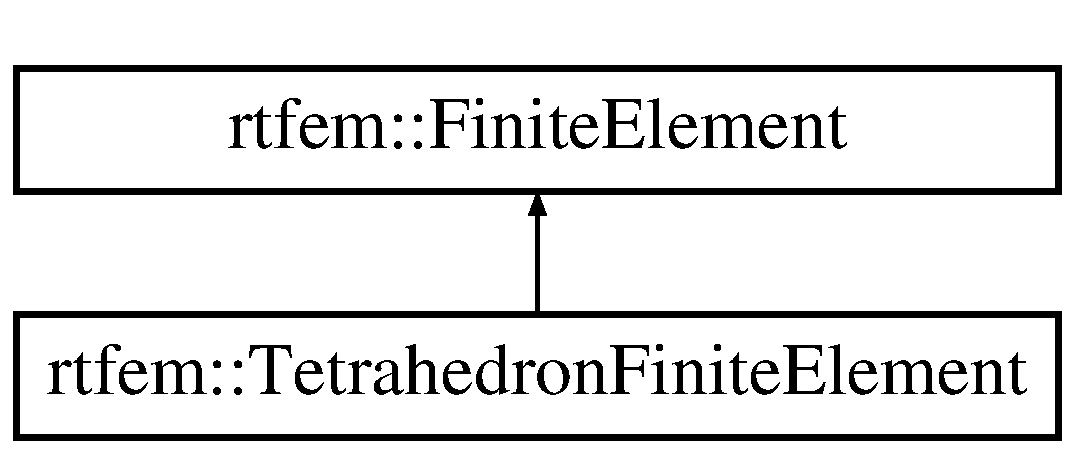
\includegraphics[height=2.000000cm]{classrtfem_1_1TetrahedronFiniteElement}
\end{center}
\end{figure}
\subsection*{Public Member Functions}
\begin{DoxyCompactItemize}
\item 
\mbox{\Hypertarget{classrtfem_1_1TetrahedronFiniteElement_a0f0d0a29e70d89424db4dfdb5dd6bb76}\label{classrtfem_1_1TetrahedronFiniteElement_a0f0d0a29e70d89424db4dfdb5dd6bb76}} 
{\bfseries Tetrahedron\+Finite\+Element} (std\+::shared\+\_\+ptr$<$ \hyperlink{classrtfem_1_1Vertex}{Vertex} $>$ vertex1, std\+::shared\+\_\+ptr$<$ \hyperlink{classrtfem_1_1Vertex}{Vertex} $>$ vertex2, std\+::shared\+\_\+ptr$<$ \hyperlink{classrtfem_1_1Vertex}{Vertex} $>$ vertex3, std\+::shared\+\_\+ptr$<$ \hyperlink{classrtfem_1_1Vertex}{Vertex} $>$ vertex4)
\item 
\mbox{\Hypertarget{classrtfem_1_1TetrahedronFiniteElement_adb2b8513f18dd6b24a63893e9f930ced}\label{classrtfem_1_1TetrahedronFiniteElement_adb2b8513f18dd6b24a63893e9f930ced}} 
U\+Int {\bfseries Get\+Vertex\+Count} () const override
\end{DoxyCompactItemize}
\subsection*{Additional Inherited Members}


The documentation for this class was generated from the following files\+:\begin{DoxyCompactItemize}
\item 
/home/samba/ciecierskij/programming/rt\+\_\+fem/sources/include/\+R\+T\+F\+E\+M/\+F\+E\+M/\+Finite\+Elements/Tetrahedron\+Finite\+Element.\+h\item 
/home/samba/ciecierskij/programming/rt\+\_\+fem/sources/src/\+R\+T\+F\+E\+M/\+F\+E\+M/\+Finite\+Elements/Tetrahedron\+Finite\+Element.\+cpp\end{DoxyCompactItemize}

\hypertarget{classrtfem_1_1TetrahedronSolver}{}\section{rtfem\+:\+:Tetrahedron\+Solver Class Reference}
\label{classrtfem_1_1TetrahedronSolver}\index{rtfem\+::\+Tetrahedron\+Solver@{rtfem\+::\+Tetrahedron\+Solver}}


{\ttfamily \#include $<$Tetrahedron\+Solver.\+h$>$}

Inheritance diagram for rtfem\+:\+:Tetrahedron\+Solver\+:\begin{figure}[H]
\begin{center}
\leavevmode
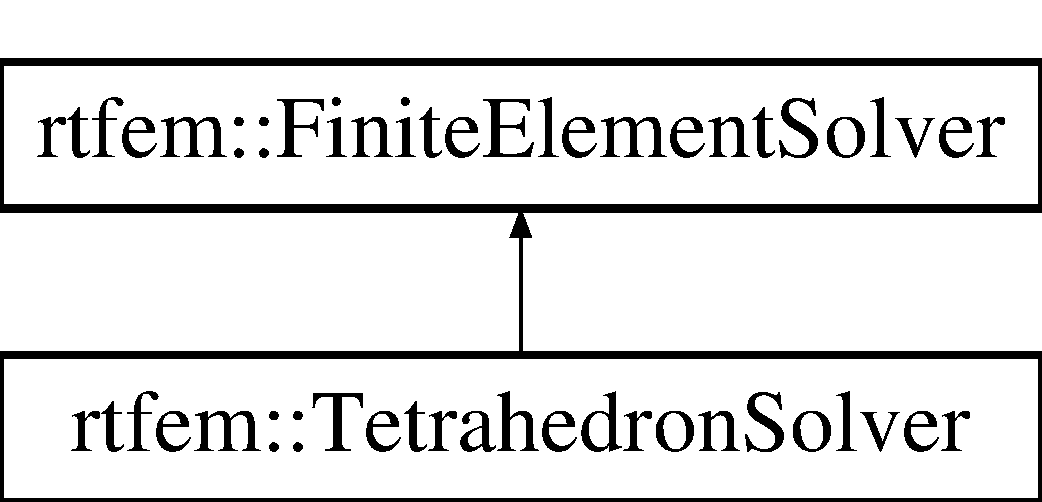
\includegraphics[height=2.000000cm]{classrtfem_1_1TetrahedronSolver}
\end{center}
\end{figure}
\subsection*{Public Member Functions}
\begin{DoxyCompactItemize}
\item 
\mbox{\Hypertarget{classrtfem_1_1TetrahedronSolver_a8d51da2dea70e926dd0975bc2ce92c52}\label{classrtfem_1_1TetrahedronSolver_a8d51da2dea70e926dd0975bc2ce92c52}} 
virtual \hyperlink{structrtfem_1_1FiniteElementSolverData}{Finite\+Element\+Solver\+Data} {\bfseries Solve} (std\+::shared\+\_\+ptr$<$ \hyperlink{classrtfem_1_1FiniteElement}{Finite\+Element} $>$ finite\+\_\+element) override
\end{DoxyCompactItemize}


\subsection{Detailed Description}
Solver for Linear Tetrahedron (constant gradient of shape function). The geometry matrix B is constant with respect to X (and always will be constant, independent of material/strain equations

Solver Data\+: Shape \hyperlink{classrtfem_1_1Matrix}{Matrix}\+: \mbox{[}3 x 12\mbox{]} Used in computing Force vector

Geometry matrix\+: \mbox{[}6 x 12\mbox{]} (Shape function gradient) Used in computing Stiffness \hyperlink{classrtfem_1_1Matrix}{Matrix} 

The documentation for this class was generated from the following files\+:\begin{DoxyCompactItemize}
\item 
/home/samba/ciecierskij/programming/rt\+\_\+fem/sources/include/\+R\+T\+F\+E\+M/\+F\+E\+M/\+Solver/\+Finite\+Element\+Solvers/Tetrahedron\+Solver.\+h\item 
/home/samba/ciecierskij/programming/rt\+\_\+fem/sources/src/\+R\+T\+F\+E\+M/\+F\+E\+M/\+Solver/\+Finite\+Element\+Solvers/Tetrahedron\+Solver.\+cpp\end{DoxyCompactItemize}

\hypertarget{structrtfem_1_1Vector3}{}\section{rtfem\+:\+:Vector3 Struct Reference}
\label{structrtfem_1_1Vector3}\index{rtfem\+::\+Vector3@{rtfem\+::\+Vector3}}
\subsection*{Public Member Functions}
\begin{DoxyCompactItemize}
\item 
\mbox{\Hypertarget{structrtfem_1_1Vector3_abec75a38bc889cc7273d3c1c0a621bf4}\label{structrtfem_1_1Vector3_abec75a38bc889cc7273d3c1c0a621bf4}} 
{\bfseries Vector3} (Float x, Float y, Float z)
\end{DoxyCompactItemize}
\subsection*{Public Attributes}
\begin{DoxyCompactItemize}
\item 
\mbox{\Hypertarget{structrtfem_1_1Vector3_aea27ef39c4e58a66805a76e1deb3b327}\label{structrtfem_1_1Vector3_aea27ef39c4e58a66805a76e1deb3b327}} 
Float {\bfseries x}
\item 
\mbox{\Hypertarget{structrtfem_1_1Vector3_abb1fbc315645530836cead78c7f4b989}\label{structrtfem_1_1Vector3_abb1fbc315645530836cead78c7f4b989}} 
Float {\bfseries y}
\item 
\mbox{\Hypertarget{structrtfem_1_1Vector3_a1cfbad91bdd38c76214eb6d4c584e931}\label{structrtfem_1_1Vector3_a1cfbad91bdd38c76214eb6d4c584e931}} 
Float {\bfseries z}
\end{DoxyCompactItemize}


The documentation for this struct was generated from the following files\+:\begin{DoxyCompactItemize}
\item 
/home/samba/ciecierskij/programming/rt\+\_\+fem/sources/include/\+R\+T\+F\+E\+M/\+Data\+Structure/Vector3.\+h\item 
/home/samba/ciecierskij/programming/rt\+\_\+fem/sources/src/\+R\+T\+F\+E\+M/\+Data\+Structure/Vector3.\+cpp\end{DoxyCompactItemize}

\hypertarget{classrtfem_1_1Vertex}{}\section{rtfem\+:\+:Vertex Class Reference}
\label{classrtfem_1_1Vertex}\index{rtfem\+::\+Vertex@{rtfem\+::\+Vertex}}
\subsection*{Public Member Functions}
\begin{DoxyCompactItemize}
\item 
\mbox{\Hypertarget{classrtfem_1_1Vertex_af617944ad95bfed3c365658b4f6206b6}\label{classrtfem_1_1Vertex_af617944ad95bfed3c365658b4f6206b6}} 
{\bfseries Vertex} (U\+Int id, const \hyperlink{structrtfem_1_1Vector3}{Vector3} \&\&cooridnates)
\item 
\mbox{\Hypertarget{classrtfem_1_1Vertex_a31414c1e1a737f47142462a79861b46c}\label{classrtfem_1_1Vertex_a31414c1e1a737f47142462a79861b46c}} 
U\+Int {\bfseries id} () const
\item 
\mbox{\Hypertarget{classrtfem_1_1Vertex_a5275104d2d988c1eb4f8796782a0010b}\label{classrtfem_1_1Vertex_a5275104d2d988c1eb4f8796782a0010b}} 
const \hyperlink{structrtfem_1_1Vector3}{Vector3} \& {\bfseries coordinates} () const
\end{DoxyCompactItemize}


The documentation for this class was generated from the following files\+:\begin{DoxyCompactItemize}
\item 
/home/samba/ciecierskij/programming/rt\+\_\+fem/sources/include/\+R\+T\+F\+E\+M/\+F\+E\+M/Vertex.\+h\item 
/home/samba/ciecierskij/programming/rt\+\_\+fem/sources/src/\+R\+T\+F\+E\+M/\+F\+E\+M/Vertex.\+cpp\end{DoxyCompactItemize}

%--- End generated contents ---

% Index
\backmatter
\newpage
\phantomsection
\clearemptydoublepage
\addcontentsline{toc}{chapter}{Index}
\printindex

\end{document}
